\chapter{Result} \label{result}

\commento{\begin{itemize}
\item asymemtries on carbon.
\item expected rates on lead.
\item false asymmetriies result.
\item average of the asymmetries for the pmts.
\item confront with the theory.
\end{itemize}}

In this chapter we report the result obtained for the data-analysis. First we report the averaged asymmetries with and without subtracting the pmt offset. From the asymmetry results, we can compute the factor $c$ as the ratio between the final asymmetries with and without subtracting the offset. The values can be directly confronted with the ones defined in \ref{Autocalib}. We see a good agreement. All the values are in reported in ppm (part-per-million).

\begin{table}[!ht]
\centering
\subfloat[][\emph{Asimmetries, with offset not subtracted.} \label{table:NotCorrected}]{ 
\begin{tabular}{c|c|c}
\hline
 PMT   &   Average &   $\sigma$ \\
\hline
 B0    &    -19.85 &      8.1 \\
 B1    &    -18.49 &      8.1 \\
 B2    &    -23.93 &      9.1 \\
 A0    &     16.66 &      3.8 \\
 A1    &     13.55 &      3.6 \\
 A2    &     16.82 &      3.9 \\
 A3    &     16.88 &      4.4 \\
 A4    &     19.48 &      5.2 \\
 A5    &     20.79 &      5.2 \\
 A6    &     17.53 &      5.7 \\
 A7    &     16.77 &      6.9 \\
\hline
\end{tabular}} \qquad
\subfloat[][\emph{Asymmetries with offsets subtracted}\label{table:OffsetCorrected}]{
\begin{tabular}{lrr} 
\hline
 PMT   &   Average &   \sigma \\
\hline
 B0    &    -19.85 &      8.1 \\
 B1    &    -18.49 &      8.1 \\
 B2    &    -23.93 &      9.1 \\
 A0    &     16.66 &      3.8 \\
 A1    &     13.55 &      3.6 \\
 A2    &     16.82 &      3.9 \\
 A3    &     16.88 &      4.4 \\
 A4    &     19.48 &      5.2 \\
 A5    &     20.79 &      5.2 \\
 A6    &     17.53 &      5.7 \\
 A7    &     16.77 &      6.9 \\
\hline
\end{tabular}}
\qquad
\subfloat[][\emph{$c$ factor, as defined in \ref{eq:Systematic}} \label{table:Cfactor}]{
\begin{tabular}{c|c} 
\hline
 PMT   &        c \\
\hline
 B0    & 0.97 \\
 B1    & 0.98 \\
 B2    & 0.99 \\
 A0    & 0.76 \\
 A1    & 0.71 \\
 A2    & 0.75 \\
 A3    & 0.8  \\
 A4    & 0.85 \\
 A5    & 0.86 \\
 A6    & 0.87 \\
 A7    & 0.91 \\
\hline
\end{tabular}}
\caption{Averaged asymmetries over all the events. The values are corrected subtracting $\overline{A}_{I}$ and considering the effective polarization $p$ of the beam}
\end{table}

The asymmetries are shown with the errors in the following plot. The error are obtained with the formula:
\begin{align*}
\sigma = \sqrt{\frac{1}{2 N \cdot n}}
\end{align*}

To Obtain a final asymmetry for detector A and B, the asymmetries for each plot are averaged using the formula:

\begin{equation}
\overline{A_{n}} = \sum_{i = 0}^{n_{PMT}} \dfrac{ w_{i} A_{i}}{\sum_{i = 0}^{n_{PMT}} w_{i}}
\end{equation}

This is a weighted mean, and $w_{i} = \frac{1}{\sigma^{2}_{i}}$. This formula is applied to take care of the different statistical error for different pmts.

\begin{figure}[hbtp]
\centering
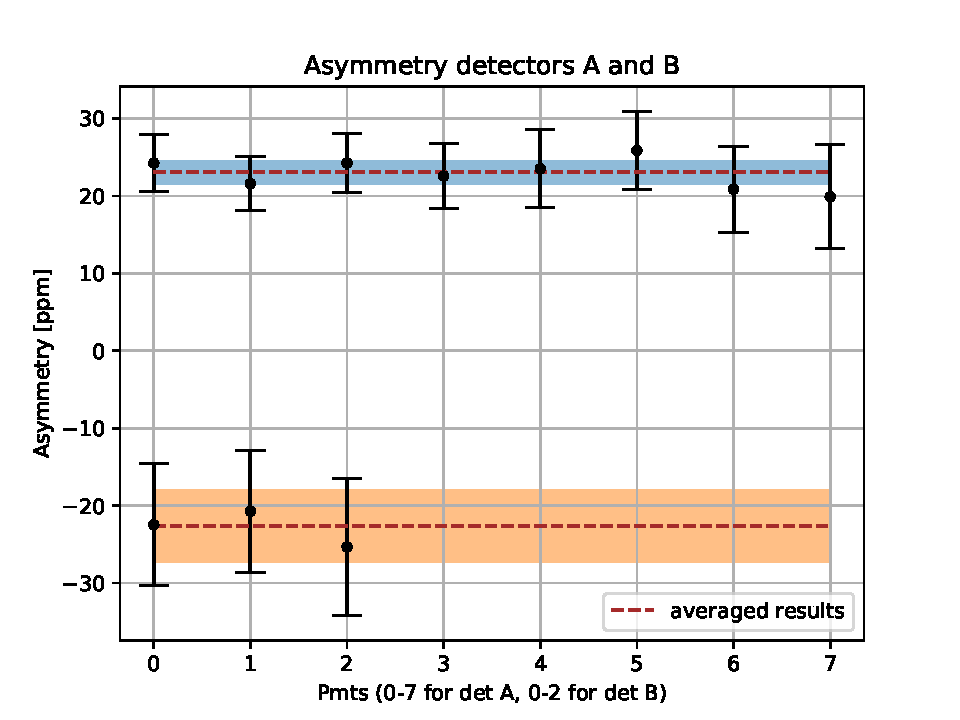
\includegraphics[width = 0.80\textwidth]{Analysis/Dataselection/FirstResult.pdf}
\caption{Plot of the asymmetries ordered by the pmt label, the result are the average event per event, corrected by the beam asymmetry current and for the polarization $p$ percentage.}
\end{figure}

The overall results for the two detectors are: 
\begin{itemize}
\item Asymmetry for detector A, $A_{A} =  23.1 \pm 1.6$ ppm.
\item Asymmetry for detector B, $A_{B} = -22.7 \pm 4.7$ ppm.
\end{itemize}

The result obtained from the linear fit are reported here. In this case the model is quite simple: only $X$, $Y$, $E$ are the beam parameters considered:
\begin{table}[h]
\centering
\begin{tabular}{|c|c|c|c|c|}
\hline
 PMT   & An             & Ax              & Ay                 & Ae              \\
\hline
 A0    & 22.19 $\pm$ 4.23 & 45.21 $\pm$ 23.74 & -66.05 $\pm$ 115.92  & 21.97 $\pm$ 9.73  \\
 A1    & 18.67 $\pm$ 4.06 & 3.55 $\pm$ 22.77  & -154.05 $\pm$ 111.2  & 24.09 $\pm$ 9.33  \\
 A2    & 21.49 $\pm$ 4.19 & -0.66 $\pm$ 23.51 & -199.85 $\pm$ 114.83 & 13.51 $\pm$ 9.63  \\
 A3    & 20.79 $\pm$ 4.44 & 21.82 $\pm$ 24.91 & -202.59 $\pm$ 121.63 & 0.73 $\pm$ 10.21  \\
 A4    & 23.19 $\pm$ 4.72 & 48.67 $\pm$ 26.49 & -158.39 $\pm$ 129.36 & 11.1 $\pm$ 10.85  \\
 A5    & 24.38 $\pm$ 4.76 & 46.55 $\pm$ 26.74 & 62.56 $\pm$ 130.58   & 3.29 $\pm$ 10.96  \\
 A6    & 19.37 $\pm$ 5.12 & -2.92 $\pm$ 28.77 & 98.39 $\pm$ 140.47   & 9.69 $\pm$ 11.79  \\
 A7    & 18.28 $\pm$ 5.77 & 5.12 $\pm$ 32.41  & 176.06 $\pm$ 158.25  & 16.92 $\pm$ 13.28 \\
\hline
\end{tabular}
\end{table}


\chapter{Conclusion and outlook} \label{conclusion}

\commento{\begin{itemize}
\item outlook for the future experiments with lead.
\item mention the future experiment with Parity-violatin scattering.
\end{itemize}}